\documentclass[]{itmo-student-thesis}

%% Опции пакета:
%% - specification - если есть, генерируется задание, иначе не генерируется
%% - annotation - если есть, генерируется аннотация, иначе не генерируется
%% - times - делает все шрифтом Times New Roman, требует пакета pscyr.

%% Делает запятую в формулах более интеллектуальной, например: 
%% $1,5x$ будет читаться как полтора икса, а не один запятая пять иксов. 
%% Однако если написать $1, 5x$, то все будет как прежде.
\usepackage{icomma}

%% Данные пакеты необязательны к использованию в бакалаврских/магистерских
%% Они нужны для иллюстративных целей
%% Начало
\usepackage{tikz}
\usetikzlibrary{arrows}
\usepackage{filecontents}
\begin{filecontents}{thesis.bib}
@article{ vyatkin-controllers,
  author      = {Yan, J. and Vyatkin, V.},
  title       = {Distributed Software Architecture Enabling Peer to Peer Communicating Controllers},
  journal     = {IEEE Transactions on Industrial Informatics},
  number      = {9(4)},
  year        = {2013},
  pages       = {2200-2209},
  langid      = {english}
}

@article{ deepmind-dqn-orig,
  author      = {Mnih, V. and others},
  title       = {Human-level control through deep reinforcement learning},
  journal     = {Nature},
  number      = {518},
  year        = {2015},
  pages       = {529-533},
  langid      = {english}
}

@article{ q-routing-orig,
  author      = {Boyan, J. A. and Littman, M. L.},
  title       = {Packet routing in dynamically changing networks: a reinforcement learning approach},
  journal     = {Advances in Neural Information Processing Systems},
  number      = {6},
  year        = {1994},
  pages       = {671-678},
  langid      = {english}
}

@article{ predictive-q-routing,
  author      = {Choi, S. P . M. and Yeung, D.-Y.},
  title       = {Predictive Q-Routing: A Memory-based Reinforcement Learning Approach to Adaptive Traffic Control},
  journal     = {Advances in Neural Information Processing Systems},
  number      = {8},
  year        = {1996},
  pages       = {945-951},
  langid      = {english}
}

@article{ dual-q-routing,
  author      = {Kumar, S. and Miikkulainen, R.},
  title       = {Dual reinforcement Q-routing: An on-line adaptive routing algorithm},
  journal     = {Artificial Neural Networks in Engineering},
  number      = {7},
  year        = {1997},
  pages       = {231-238},
  langid      = {english}
}

@phdthesis{ q-learning-orig,
    title    = {Learning from Delayed Rewards},
    school   = {King's College},
    address  = {Cambridge},
    author   = {Watking, C.},
    year     = {1989}
}

@article{ link-state-arpanet,
  author      = {McQuillan, J. M. and Richer, I. and Rosen, E. C.},
  title       = {The New Routing Algorithm for the ARPANet},
  journal     = {IEEE Trans. on Comm.},
  number      = {28(5)},
  year        = {1980},
  pages       = {711–719}
}

@article{ arpanet-orig,
  author      = {McQuillan, J. M. and Walden, D. C.},
  title       = {The ARPA network design decisions},
  journal     = {Computer Networks},
  number      = {1(5)},
  year        = {1977},
  pages       = {243-289}
}

@techreport{ rip-rfc,
  AUTHOR = {Hendrick, C.},
  TITLE = {Routing Information Protocol},
  TYPE= {RFC},
  NUMBER = {1058},
  YEAR = {1988},
  MONTH = {June},
}

@techreport{ ospf-rfc,
  AUTHOR = {Moy, J.},
  TITLE = {OSPF Version 2},
  TYPE = {RFC},
  NUMBER = 1058,
  YEAR = {1998},
  MONTH = {April},
}

@misc{ igrp-patent,
  title={Method and apparatus for routing communications among computer networks},
  author={Bosack, L.},
  url={https://www.google.com/patents/US5088032},
  year={1992},
  month=feb # "~11",
  publisher={Google Patents},
  note={US Patent 5,088,032}
}

@article{ bellman-ford,
  author = {Bellman, Richard},
  title = {On a routing problem},
  journal = {Quarterly of Applied Mathematics},
  number = {16},
  year = {1958},
  pages = {87-90}
}

@article{ dijkstra,
  author = {Dijkstra, E. W.},
  title = {A note on two problems in connexion with graphs},
  journal = {Numerische Mathematik},
  number = {1},
  year = {1959},
  pages = {269-271}
}
\end{filecontents}
%% Конец

%% Указываем файл с библиографией.
\addbibresource{thesis.bib}

%% Всякая фигня
\DeclareMathOperator{\argmin}{argmin}

\begin{document}

\studygroup{M3438}
\title{Глубокие самообучающиеся агенты для мультиагентной системы маршрутизации}
\author{Мухутдинов Дмитрий Вадимович}{Мухутдинов Д.В.}
\supervisor{Фильченков Андрей Александрович}{Фильченков А.А.}{к.ф.-м.н}{доцент кафедры КТ}
\publishyear{2017}
%% Дата выдачи задания. Можно не указывать, тогда надо будет заполнить от руки.
\startdate{01}{сентября}{2016}
%% Срок сдачи студентом работы. Можно не указывать, тогда надо будет заполнить от руки.
\finishdate{31}{мая}{2017}
%% Дата защиты. Можно не указывать, тогда надо будет заполнить от руки.
%% \defencedate{15}{июня}{2015}

\addconsultant{Вяткин В.В.}{PhD, Luleå University of Technology}

%% Задание
%%% Техническое задание и исходные данные к работе
\technicalspec{
  Требуется разработать алгоритм решения обобщенной задачи маршрутизации, основанный на идее мультиагентного обучения нейронных сетей с подкреплением.
  Требуется применить метод к решению конкретных задач маршрутизации, таких как маршрутизация сетевых пакетов и управление конвейерной системой
  транспортировки багажа, и сравнить его c существующими алгоритмами.
}

%%% Содержание выпускной квалификационной работы (перечень подлежащих разработке вопросов)
\plannedcontents{
  \begin{enumerate}
  \item Обзор предметной области
  \item Реализация среды для эмуляции задачи сетевой маршрутизации
  \item Реализация среды для эмуляции конвейерной системы транспортировки багажа
  \item Разработка алгоритма маршрутизации на основе мультиагентного обучения нейронных сетей с подкреплением
  \item Реализация существующих алгоритмов решения задач маршрутизации
  \item Проведение экспериментов, интерпретация результатов
  \end{enumerate}
}

%%% Исходные материалы и пособия 
\plannedsources{\begin{enumerate}
    \item Richard S. Sutton and Andrew G. Barto. Reinforcement Learning: An Introduction. The MIT Press, 2012
    \item Mnih et al. Human-level control through deep reinforcement learning. Nature, 518(7540):529–533, 2015.
\end{enumerate}}

%%% Календарный план
\addstage{Ознакомление с предметной областью}{11.2016}
\addstage{Чтение статей, посвященных алгоритмам маршрутизации}{12.2016}
\addstage{Чтение статей, посвященных задаче обучения с подкреплением}{01.2017}
\addstage{Разработка сред для эмуляции задач маршрутизации}{03.2017}
\addstage{Разработка алгоритма маршрутизации, реализация существующих алгоритмов}{04.2017}
\addstage{Проведение экспериментов, написание пояснительной записки}{05.2017}

%%% Цель исследования
\researchaim{
  Разработка распределенного алгоритма решения задачи маршрутизации, подходящего для
  эффективного применения в различных условиях, включая киберфизические системы.
}

%%% Задачи, решаемые в ВКР
\researchtargets{\begin{enumerate}
    \item Формальная постановка обобщенной задачи маршрутизации.
    \item Разработка алгоритма решения поставленной задачи.
    \item Сравнение работы алгоритма с существующими решениями на практике.
\end{enumerate}}

%%% Использование современных пакетов компьютерных программ и технологий
\advancedtechnologyusage{
  Для решения задачи использовался язык программирования Python.
  При разработке систем эмуляции работы компьютерной сети и системы управления
  багажными конвейерами была использована библиотека Thespian. Для реализации и
  обучения нейронных сетей были использованы библиотеки TensorFlow и Keras.
}

%%% Краткая характеристика полученных результатов 
\researchsummary{
  Разработана формальная постановка обобщенной задачи маршрутизации в терминах
  мультиагентного обучения с подкреплением. Разработан алгоритм решения
  обобщенной задачи маршрутизации. Разработанный алгоритм по результатам
  экспериментов на практике не уступает современным специализированным
  алгоритмам решения задач сетевого роутинга и управления конвейерной системой,
  но благодаря обобщенной постановке задачи и применению нейронных
  сетей имеет широкий потенциал применения для решения задач, сводимых к задаче
  маршрутизации, в сложных условиях (таких, как киберфизические системы).
}

%%% Гранты, полученные при выполнении работы 
\researchfunding{
  При выполнении работы грантов получено не было.
}

%%% Наличие публикаций и выступлений на конференциях по теме выпускной работы
\researchpublications{
  По теме данной работы публикаций и выступлений на конференциях нет.
}

\graphicspath{{img/}}

%% Эта команда генерирует титульный лист и аннотацию.
\maketitle{Бакалавр}

%% Оглавление
\tableofcontents

%% Макрос для введения. Совместим со старым стилевиком.
\startprefacepage

Задача пакетной маршрутизации - это задача поиска кратчайшего пути в графе в условиях,
когда за каждый узел графа отвечает отдельный вычислительный процесс. Это
означает, что каждый отдельный узел графа должен принять решение о том, какому
из соседей следует отправить очередной пакет, чтобы тот достиг пункта назначения
как можно быстрее.

Задача пакетной маршрутизации впервые обрела актуальность с появлением
компьютерных сетей. Первые алгоритмы сетевой маршрутизации появились в процессе
разработки сети ARPANet. Именно тогда были изобретены такие подходы к пакетной
маршрутизации, как distance-vector\cite{arpanet-orig} и
link-state\cite{link-state-arpanet}, которые и по сей день лежат в основе таких
стандартных и широко применяемых алгоритмов сетевой маршрутизации, как Routing
Information Protocol (RIP)\cite{rip-rfc} и Open Shortest Path First (OSPF)\cite{ospf-rfc}.

Оба этих подхода основаны на идее вычисления кратчайшего пути между текущим
узлом сети и пунктом назначения пакета. Однако существуют и другие подходы к
решению задачи маршрутизации, основанные на идее обучения с подкреплением
(reinforcement learing). Первым таким алгоритмом стал алгоритм
Q-routing\cite{q-routing-orig}, основанный на методе
Q-learning\cite{q-learning-orig}. Этот алгоритм, как и его
модификации\cite{predictive-q-routing, dual-q-routing},
благодаря обучению с подкреплением оказался способен лучше адаптироваться к
изменениям в интенсивности сетевого трафика, чем алгоритмы, основанные на
вычислении кратчайшего пути, но из-за использования большего количества
служебных сообщений применение таких алгоритмов в реальных сетях ограничено.

Но стоит отметить, что задача маршрутизации встречается не только в компьютерных сетях, но
также и в более сложных средах, таких как киберфизические системы. Примером такой
задачи, частично решаемой с помощью алгоритмов маршрутизации, является
управление конвейерной системой (в частности, системой распределения багажа в
аэропорту). Задача управления такой системой в большинстве случаев решается с
помощью централизованных алгоритмов, и децентрализованное решение (основанное на
алгоритма Беллмана-Форда) было предложено совсем недавно\cite{vyatkin-controllers}. 
Такая задача отличается от задачи сетевого роутинга, с одной
стороны, тем, что служебные сообщения и целевые сообщения являются разными
сущностями (``целевое сообщение'' --- это чемодан, а служебные сообщения являются
цифровыми), и служебные сообщения передаются мгновенно по сравнению с целевыми.
С другой стороны, состояние каждого конвейера и всей системы в целом задается
большим количеством параметров --- такими как скорости конвейеров, положение,
количество и масса чемоданов на каждом конвейере, и так далее. С третьей
стороны, желательно, чтобы система оптимизировала не только скорость доставки
чемоданов до точки назначения, но и, к примеру, собственное энергопотребление.

Первое обстоятельство снимает технические ограничения на количество служебных
сообщений, что позволяет в полной мере применять алгоритмы на основе обучения с
подкреплением. Второе и третьи обстоятельства усложняют написание оптимального
детерминированного алгоритма и наталкивают на идею реализации приближенного
решения, например, с использованием нейронных сетей.

В настоящее время в области обучения с подкреплением с применением нейронных
сетей достигнуты впечатляющие успехи. Всплеск активности в этой области
произошел после выхода статьи команды Google DeepMind об обучении глубокой
сверточной нейронной сети игре на консоли Atari 2600\cite{deepmind-dqn-orig}.
Применению полученной модели к различным задачам в различных условиях посвящено
множество исследований, часть из них посвящена проблеме мультиагентного обучения
с подкреплением (multi-agent reinforcement learning). Так как задачу
маршрутизации можно сформулировать как задачу мультиагентного обучения с
подкреплением, имеет смысл применить данные наработки для ее решения.

В данной работе будет предложен алгоритм маршрутизации, основанный на методе
Q-routing, но использующий нейронную сеть в качестве обучающегося агента.
На данный момент не существует алгоритма маршрутизации, построенного по такому
принципу.

В главе 1 будет сформулирована обобщенная постановка задачи маршрутизации в
терминах мультиагентного обучения с подкреплением. Будут рассмотрены
существующие алгоритмы маршрутизации, их сильные и слабые стороны. Также будут
рассмотрены существующие методы обучения нейронных сетей с подкреплением, в том
числе в мультиагентном случае.

В главе 2 будет рассмотрен предложенный алгоритм и обоснованы решения, принятые
в ходе его разработки.

В главе 3 будут приведены экспериментальные результаты работы алгоритма для
задач пакетной маршрутизации в компьютерной сети и управления системой багажных
конвейеров. Будут приведены результаты работы в условиях неравномерной
нагрузки на сеть (или конвейерную систему) и изменения топологии сети. Также
будет проведено сравнение с существующими алгоритмами маршрутизации.

%% Начало содержательной части.
\chapter{Обзор предметной области}

\section{Постановка задачи}
Пусть задана сеть в виде графа: $G = (V, E)$. Каждому узлу и каждому ребру в сети
приписывается некоторое \textit{состояние}: узел v имеет состояние $s_v \in S_V$, ребро e
имеет состояние $s_e \in S_E$. Состояние всей сети, таким образом, описывается как
$s = (s_{v_1}, ... , s_{v_n}, s_{e_1}, ... , s_{e_m}) \in S$.

На узел сети $s \in V$ приходят пакеты $p = (d, prop)$, где $d \in V$ - узел
назначения пакета, а $prop$ - произвольная дополнительная информация о нем.
Обозначим множество всевозможных свойств пакета как $Prop$ ($prop \in Prop$), а
множество пакетов в целом, таким образом, как $P = (V, Prop)$. Также заданы
некоторые функции \textit{стоимости} прохождения данного пакета через ребра и
узлы сети, зависящие от их состояний:
$R_v : V \times S_V \times P \rightarrow \Bbb{R}^+$ - стоимость прохождения
пакета через узел, $R_e : E \times S_E \times P \rightarrow \Bbb{R}^+$. Мы явно
указываем, что стоимости неотрицательны, чтобы избежать таких постановок задач,
в которых существуют пути стоимости $-\infty$ (циклы отрицательной стоимости).

Задача пакетной маршрутизации заключается в том, чтобы определить, какому из
соседей $n \in \{v | (s, v) \in E\}$ узел $s$ должен перенаправить пакет
$p = (d, prop)$, чтобы ожидаемая стоимость пути от $s$ до $d$ была минимальной.

\section{Существующие алгоритмы маршрутизации}

Почти все существующие алгоритмы маршрутизации были разработаны для
маршрутизации пакетов в компьютерных сетях. Большинство алгоритмов маршрутизации
в компьютерных сетях, применяемых на практике, относятся к одному из двух
семейств алгоритмов --- дистанционно-векторные (distance-vector)\cite{arpanet-orig} или
состояния каналов связи (link-state)\cite{link-state-arpanet}.
Концептуально все алгоритмы внутри каждого из этих семейств одинаковы, и различаются только
техническими деталями реализации, обусловленными спецификой конкретной узкой
сферы применения. Поэтому мы не будем рассматривать алгоритмы каждого семейства
по отдельности, а рассмотрим только концепции в целом.

\subsection{Дистанционно-векторные алгоритмы}

Идея дистанционно-векторных алгоритмов (distance-vector algoritms) заключается в
следующем:

\begin{itemize}
\item Каждый маршрутизатор $s$ в сети хранит таблицу, в которой для каждого другого узла
  сети $d$ хранится следующая информация:
  \begin{itemize}
  \item Предполагаемое кратчайшее расстояние от $s$ до $d$
  \item Сосед $n$, которому нужно отправить пакет, чтобы пакет прошел по
    кратчайшему пути до узла $d$.
  \end{itemize}
\item Периодически каждый маршрутизатор рассылает свою версию таблицы кратчайших
  расстояний всем своим соседям
\item При получении вектора кратчайших расстояний от соседа маршрутизатор $s$
  сравнивает его поэлементно с текущей версией. Если оказывается, что наименьшая
  стоимость пути от соседа $n$ до узла $d$, сложенная c оценкой стоимости ребра
  $(s, d)$ меньше, чем наименьшая стоимость пути от $s$ до $d$ в текущей
  таблице, то значение в текущей таблице обновляется, и наилучшим соседом для
  отправки пакета в узел $d$ становится сосед $n$.
\end{itemize}

Как можно видеть, дистанционно-векторный алгоритм является, в сущности,
распределенной версией алгоритма Беллмана-Форда поиска кратчайшего пути в
графе\cite{bellman-ford}.

\begin{figure}[!h]
  \caption{Иллюстрация работы distance-vector алгоритма}\label{rip-img}
  \centering
  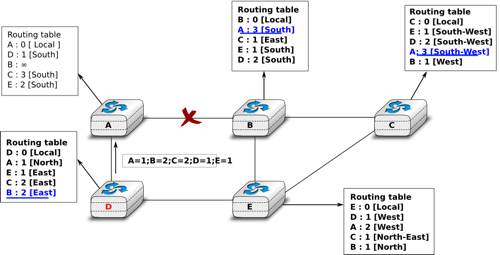
\includegraphics[scale=1.5]{dv-failure-2}
\end{figure}

Различные реализации дистанционно-векторного метода различаются, в частности,
оценками стоимости соединений в сети. Так, например, протокол RIP\cite{rip-rfc} просто
оценивает стоимость каждого соединения в 1, а IGRP\cite{igrp-patent} оценивает
стоимость соединений исходя из оценок задержки и пропускной способности.

Преимуществами дистанционно-векторных алгоритмов являются простота реализации и
низкие требования к памяти и вычислительной мощности. Недостатками же являются
низкая скорость распространения информации по сети и сложности с приспособлением
под изменяющуюся топологию (проблема count-to-infinity). Этих проблем
удается избежать при применении другого распространенного подхода - алгоритмов
на основе состояния канала связи. 

\subsection{Алгоритмы состояния канала связи}

В отличие от дистанционно-векторных алгоритмов, в алгоритмах состояния канала связи
(link-state) каждый узел сети хранит у себя модель всей сети в виде графа.
Рассмотрим шаги алгоритма подробнее:

\begin{itemize}
\item Каждый маршрутизатор периодически проверяет состояние соединений до
  соседей
\item При обнаружении обрыва какого-либо соединения алгоритм удаляет это
  соединение из собственного графа и рассылает соседям новую версию состояния
  соединений до них
\item Соседи обновляют собственные версии графов в соответствии с полученной
  информацией и пересылают сообщение дальше
\item Чтобы избежать зацикливания сообщений об обновлении состояния, каждое
  сообщение снабжается \textit{номером версии}. Маршрутизатор $n$ игнорирует
  сообщение от маршрутизатора $n$, если номер версии этого сообщения меньше или
  равен предыдущему.
\end{itemize}

\begin{figure}[!h]
  \caption{Иллюстрация работы link-state алгоритма}\label{ospf-img}
  \centering
  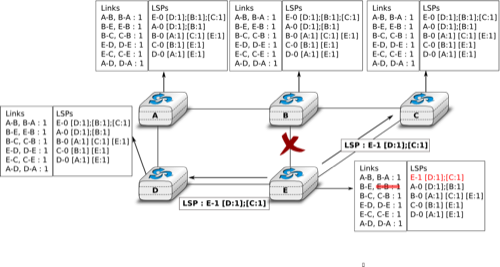
\includegraphics[scale=1.5]{ls-twoway}
\end{figure}

Имея информацию обо всей сети в целом, маршрутизатор может рассчитать кратчайшие
пути до всех остальных узлов. Обычно для этого используется алгоритм
Дейкстры\cite{dijkstra}. 

Link-state алгоритмы обладают способностью адаптироваться под изменения
топологии сети гораздо быстрее, чем distance-vector алгоритмы за счет довольно
несколько более сложной реализации и чуть больших затрат по памяти и
вычислительной мощности. Это обуславливает то, что на данный момент именно
link-state протоколы, такие как OSPF\cite{ospf-rfc}, доминируют в сетевой
маршрутизации. Однако даже в решении задачи сетевой маршрутизации link-state
алгоритмы в чистом виде не лучшим образом адаптируются к повышению нагрузки в
сети. Рассматриваемые в дальнейшем другие алгоритмы, основанные на принципе
обучения с подкреплением, справляются с задачей адаптации к
изменчивой нагрузке лучше.

\subsection{Другие подходы}

Среди других подходов особый интерес представляют подходы на основе обучения с
подкреплением. Первым алгоритмом маршрутизации, основанным на этой идее, стал
алгоритм Q-routing\cite{q-routing-orig}. Принцип его работы таков:

\begin{itemize}
\item Каждый маршрутизатор $x$ хранит $Q_x(d, y)$ --- оценку минимального
  времени в пути до узла $d$, если следующим узлом на пути является сосед $y$.
  Очевидно, что $\forall y : Q_x(x, y) = 0$ 
\item Пакет, который необходимо доставить в узел $d$, отправляется соседу
  $y = \argmin\limits_{(x, y) \in E} Q_x(d, y)$
\item При получении пакета узел $y$ отправляет узлу $x$ время получения $t_r$ и
  собственную оценку оставшегося времени в пути
  $t = \min\limits_{(y, z) \in E} Q_y(d, z)$
\item Зная время отправления пакета $t_s$ и получив $t_r$ и $t$, узел $x$
  обновляет собственную оценку по формуле:
  $Q_x(d, y) = \alpha((t_r - t_s) + t - Q_x(d, y)) + Q_x(d, y)$,
  где $\alpha$ --- это learning rate, параметр алгоритма.
\end{itemize}

Было показано, что этот алгоритм способен хорошо адаптироваться к изменениям в
топологии сети и интенсивности трафика. Такие его модификации, как dual
Q-routing и predictive Q-routing еще более высокое качество маршрутизации.
Однако по сравнению с distance-vector или link-state методами данные алгоритмы
используют гораздо больше служебных сообщений (служебный пакет на каждую
пересылку целевого пакета), что ограничивает их применение в реальных
высоконагруженных компьютерных сетях. 

Однако в задачах маршрутизации вне контекста компьютерных сетей это перестает
быть проблемой, так как целевые ``пакеты'' (чемоданы на конвейере, автомобили на
автостраде, etc.) и служебные сообщения являются объектами разной природы и
передаются по разным каналам, причем служебные сообщения по сравнению с целевыми
``пакетами'' доставляются мгновенно. Эти обстоятельства делают применение
алгоритмов обучения с подкреплением в таких задачах более привлекательным.



\section{Термины и понятия}

\textbf{Обучение с подкреплением} - вид машинного обучения, в котором \textit{}

\begin{enumerate}
\item Множества 
\item Q-learning 
\item 
\end{enumerate}

\section{Постановка задачи в терминах обучения с подкреплением}

\section{Обзор методов обучения нейросетей с подкреплением}

\begin{table}[!h]
\caption{Таблица умножения (фрагмент)}\label{tab1}
\centering
\begin{tabular}{|*{18}{c|}}\hline
-- & 1 & 2 & 3 & 4 & 5 & 6 & 7 & 8 & 9 & 10 & 11 & 12 & 13 & 14 & 15 & 16 & 17 \\\hline
1  & 1 & 2 & 3 & 4 & 5 & 6 & 7 & 8 & 9 & 10 & 11 & 12 & 13 & 14 & 15 & 16 & 17 \\\hline
2  & 2 & 4 & 6 & 8 & 10 & 12 & 14 & 16 & 18 & 20 & 22 & 24 & 26 & 28 & 30 & 32 & 34 \\\hline
3  & 3 & 6 & 9 & 12 & 15 & 18 & 21 & 24 & 27 & 30 & 33 & 36 & 39 & 42 & 45 & 48 & 51 \\\hline
4  & 4 & 8 & 12 & 16 & 20 & 24 & 28 & 32 & 36 & 40 & 44 & 48 & 52 & 56 & 60 & 64 & 68 \\\hline
\end{tabular}
\end{table}

Есть еще такое окружение \texttt{tabu}, его можно аккуратно растянуть на всю страницу.
Приведем пример (таблица~\ref{tab2}).

\begin{table}[!h]
\caption{Таблица умножения с помощью \texttt{tabu} (фрагмент)}\label{tab2}
\centering
\begin{tabu}{|*{18}{X[c]|}}\hline
-- & 1 & 2 & 3 & 4 & 5 & 6 & 7 & 8 & 9 & 10 & 11 & 12 & 13 & 14 & 15 & 16 & 17 \\\hline
1  & 1 & 2 & 3 & 4 & 5 & 6 & 7 & 8 & 9 & 10 & 11 & 12 & 13 & 14 & 15 & 16 & 17 \\\hline
2  & 2 & 4 & 6 & 8 & 10 & 12 & 14 & 16 & 18 & 20 & 22 & 24 & 26 & 28 & 30 & 32 & 34 \\\hline
3  & 3 & 6 & 9 & 12 & 15 & 18 & 21 & 24 & 27 & 30 & 33 & 36 & 39 & 42 & 45 & 48 & 51 \\\hline
4  & 4 & 8 & 12 & 16 & 20 & 24 & 28 & 32 & 36 & 40 & 44 & 48 & 52 & 56 & 60 & 64 & 68 \\\hline
\end{tabu}
\end{table}

\section{Рисунки}

Пример рисунка (c помощью \texttt{TikZ}) приведен на рисунке~\ref{fig1}. Под \texttt{pdflatex} можно также
использовать \texttt{*.jpg}, \texttt{*.png} и даже \texttt{*.pdf}, под \texttt{latex} можно использовать
Metapost. Последний можно использовать и под \texttt{pdflatex}, для чего в стилевике продекларированы
номера картинок от~1 до~20.

\begin{figure}[!h]
\caption{Пример рисунка}\label{fig1}
\centering
\begin{tikzpicture}[scale=0.7]
\draw[thick,->] (0,0)--(3.5,0);
\draw[thick,->] (0,0)--(0,3.5);
\draw[very thick, red] (0,0)--(3,3);
\draw[dashed] (3,0)--(3,3);
\draw[dashed] (1.5,0)--(1.5,1.5);
\end{tikzpicture}
\end{figure}

\section{Листинги}

В работах студентов кафедры <<Компьютерные технологии>> часто встречаются листинги. Листинги бывают
двух основных видов~--- исходный код и псевдокод. Первый оформляется с помощью окружения \texttt{lstlisting}
из пакета \texttt{listings}, который уже включается в стилевике и немного настроен. Пример Hello World на Java
приведен на листинге~\ref{lst1}.

\begin{lstlisting}[float=!h,caption={Пример исходного кода на Java},label={lst1}]
public class HelloWorld {
	public static void main(String[] args) {
		System.out.println("Hello, world!");
	}
}
\end{lstlisting}

\subsection{Тест}

Псевдокод можно оформлять с помощью разных пакетов. В данном стилевике включается пакет \texttt{algorithmicx}.
Сам по себе он не генерирует флоатов, поэтому для них используется пакет \texttt{algorithm}.
Пример их совместного использования приведен на листинге~\ref{lst2}. Обратите внимание, что флоаты разные, а 
нумерация~--- общая!

\begin{algorithm}[!h]
\caption{Пример псевдокода}\label{lst2}
\begin{algorithmic}
	\Function{IsPrime}{$N$}
		\For{$t \gets [2; \lfloor\sqrt{N}\rfloor]$}
			\If{$N \bmod t = 0$}
				\State\Return \textsc{false}
			\EndIf
		\EndFor
		\State\Return \textsc{true}
	\EndFunction
\end{algorithmic}
\end{algorithm}

Наконец, листинги из \texttt{listings} тоже можно подвешивать с помощью \texttt{algorithm},
пример на листинге~\ref{lst3}.

\begin{algorithm}[!h]
\caption{Исходный код и флоат \texttt{algorithm}}\label{lst3}
\begin{lstlisting}
public class HelloWorld {
	public static void main(String[] args) {
		System.out.println("Hello, world!");
	}
}
\end{lstlisting}
\end{algorithm}

\chapter{Проверка сквозной нумерации}

Листинг~\ref{lst4} должен иметь номер 4.

\begin{algorithm}[!h]
\caption{Исходный код и флоат \texttt{algorithm}}\label{lst4}
\begin{lstlisting}
public class HelloWorld {
	public static void main(String[] args) {
		System.out.println("Hello, world!");
	}
}
\end{lstlisting}
\end{algorithm}

Рисунок~\ref{fig2} должен иметь номер 2.

\begin{figure}[!h]
\caption{Пример рисунка}\label{fig2}
\centering
\begin{tikzpicture}[scale=0.7]
\draw[thick,->] (0,0)--(3.5,0);
\draw[thick,->] (0,0)--(0,3.5);
\draw[very thick, red] (0,0)--(3,3);
\draw[dashed] (3,0)--(3,3);
\draw[dashed] (1.5,0)--(1.5,1.5);
\end{tikzpicture}
\end{figure}

Таблица~\ref{tab3} должна иметь номер 3.

\begin{table}[!h]
\caption{Таблица умножения с помощью \texttt{tabu} (фрагмент)}\label{tab3}
\centering
\begin{tabu}{|*{18}{X[c]|}}\hline
-- & 1 & 2 & 3 & 4 & 5 & 6 & 7 & 8 & 9 & 10 & 11 & 12 & 13 & 14 & 15 & 16 & 17 \\\hline
1  & 1 & 2 & 3 & 4 & 5 & 6 & 7 & 8 & 9 & 10 & 11 & 12 & 13 & 14 & 15 & 16 & 17 \\\hline
2  & 2 & 4 & 6 & 8 & 10 & 12 & 14 & 16 & 18 & 20 & 22 & 24 & 26 & 28 & 30 & 32 & 34 \\\hline
3  & 3 & 6 & 9 & 12 & 15 & 18 & 21 & 24 & 27 & 30 & 33 & 36 & 39 & 42 & 45 & 48 & 51 \\\hline
4  & 4 & 8 & 12 & 16 & 20 & 24 & 28 & 32 & 36 & 40 & 44 & 48 & 52 & 56 & 60 & 64 & 68 \\\hline
\end{tabu}
\end{table}

\chapterconclusion

В конце каждой главы желательно делать выводы. Вывод по данной главе~--- нумерация работает корректно, ура!

%% Макрос для заключения. Совместим со старым стилевиком.
\startconclusionpage

TBD

\printmainbibliography

%% После этой команды chapter будет генерировать приложения, нумерованные русскими буквами.
%% \startappendices из старого стилевика будет делать то же самое
\appendix

\chapter{Пример приложения}

В приложениях рисунки, таблицы и другие подобные элементы нумеруются по приложениям с соответствующим префиксом. Проверим это.

Листинг~\ref{lst4:apx} должен иметь номер А.1.

\begin{algorithm}[!h]
\caption{Исходный код и флоат \texttt{algorithm}}\label{lst4:apx}
\begin{lstlisting}
public class HelloWorld {
	public static void main(String[] args) {
		System.out.println("Hello, world!");
	}
}
\end{lstlisting}
\end{algorithm}

Рисунок~\ref{fig2:apx} должен иметь номер A.1.

\begin{figure}[!h]
\caption{Пример рисунка}\label{fig2:apx}
\centering
\begin{tikzpicture}[scale=0.7]
\draw[thick,->] (0,0)--(3.5,0);
\draw[thick,->] (0,0)--(0,3.5);
\draw[very thick, red] (0,0)--(3,3);
\draw[dashed] (3,0)--(3,3);
\draw[dashed] (1.5,0)--(1.5,1.5);
\end{tikzpicture}
\end{figure}

Таблица~\ref{tab3:apx} должна иметь номер A.1.

\begin{table}[!h]
\caption{Таблица умножения с помощью \texttt{tabu} (фрагмент)}\label{tab3:apx}
\centering
\begin{tabu}{|*{18}{X[c]|}}\hline
-- & 1 & 2 & 3 & 4 & 5 & 6 & 7 & 8 & 9 & 10 & 11 & 12 & 13 & 14 & 15 & 16 & 17 \\\hline
1  & 1 & 2 & 3 & 4 & 5 & 6 & 7 & 8 & 9 & 10 & 11 & 12 & 13 & 14 & 15 & 16 & 17 \\\hline
2  & 2 & 4 & 6 & 8 & 10 & 12 & 14 & 16 & 18 & 20 & 22 & 24 & 26 & 28 & 30 & 32 & 34 \\\hline
3  & 3 & 6 & 9 & 12 & 15 & 18 & 21 & 24 & 27 & 30 & 33 & 36 & 39 & 42 & 45 & 48 & 51 \\\hline
4  & 4 & 8 & 12 & 16 & 20 & 24 & 28 & 32 & 36 & 40 & 44 & 48 & 52 & 56 & 60 & 64 & 68 \\\hline
\end{tabu}
\end{table}

Заодно проверим нумерованные и ненумерованные перечисления. Ненумерованные:
\begin{itemize}
    \item пункт А;
    \item пункт Б;
    \item пункт В.
\end{itemize}

Нумерованные списки нескольких уровней:
\begin{enumerate}
    \item первый элемент;
    \item второй элемент с подэлементами:
    \begin{enumerate}
        \item первый подэлемент;
        \item второй подэлемент;
        \item третий подэлемент.
    \end{enumerate}
    \item третий элемент;
    \item четвертый элемент;
    \item пятый элемент;
    \item шестой элемент;
    \item седьмой элемент;
    \item восьмой элемент;
    \item девятый элемент;
    \item десятый элемент.
\end{enumerate}

\chapter{Еще один пример приложения  с неимоверно длиннющим названием для тестирования переносов}

Проверим на примере таблиц, что нумерация в приложениях~--- по приложениям.
Таблица~\ref{tab3:apx2} должна иметь номер Б.1.

\begin{table}[!h]
\caption{Таблица умножения с помощью \texttt{tabu} (фрагмент)}\label{tab3:apx2}
\centering
\begin{tabu}{|*{18}{X[c]|}}\hline
-- & 1 & 2 & 3 & 4 & 5 & 6 & 7 & 8 & 9 & 10 & 11 & 12 & 13 & 14 & 15 & 16 & 17 \\\hline
1  & 1 & 2 & 3 & 4 & 5 & 6 & 7 & 8 & 9 & 10 & 11 & 12 & 13 & 14 & 15 & 16 & 17 \\\hline
2  & 2 & 4 & 6 & 8 & 10 & 12 & 14 & 16 & 18 & 20 & 22 & 24 & 26 & 28 & 30 & 32 & 34 \\\hline
3  & 3 & 6 & 9 & 12 & 15 & 18 & 21 & 24 & 27 & 30 & 33 & 36 & 39 & 42 & 45 & 48 & 51 \\\hline
4  & 4 & 8 & 12 & 16 & 20 & 24 & 28 & 32 & 36 & 40 & 44 & 48 & 52 & 56 & 60 & 64 & 68 \\\hline
\end{tabu}
\end{table}

\end{document}
